
\chapter{Overlap in Observational Studies: Difficulties and Opportunities}
  \label{chapter::overlap}


 
\section{Implications of overlap}

In Part \ref{part::observational-studies} of this book, causal inference with observational studies relies on two critical assumptions: ignorability  
$$
Z\ind \{ Y(1), Y(0)  \} \mid X
$$
 and overlap  
 $$
 0 <  e(X) <  1 .
 $$ 
 \citet{d2017overlap} pointed out the tension between these two assumptions: typically, more covariates make the ignorability assumption more plausible (ignoring M-bias discussed in Chapter \ref{section::m-bias}), but more covariates make the overlap assumption less plausible because the treatment becomes more predictable given more covariates. 

If some units have $e(X) = 0$ or $e(X) = 1$, then we have philosophic difficulty in thinking about the counterfactual potential outcomes \citep{king2006dangers}. In particular, if a unit deterministically receives the treatment, then it may not be meaningful to conceive its potential outcome under the control; if a unit deterministically receives the control, then it may not be meaningful to conceive its potential outcome under the treatment.
Even if the true propensity score is not exactly $0$ or $1$, the estimated propensity score can be very close to $0$ or $1$ in finite samples, which makes the estimators based on IPW numerically unstable. 
I have discussed this issue in Chapter \ref{chapter::pscore-key}. 


Many statistical analyses in fact require a strict version of overlap:

\begin{assumption}
[strict overlap]
\label{assume::strong-overlap}
$\eta \leq e(X) \leq 1-\eta$ for some $\eta \in (0,1/2).$
\end{assumption}


However, \citet[][Corollary 1]{d2017overlap} showed that Assumption \ref{assume::strong-overlap} has very strong implications when the number of covariates is large. For simplicity, I present only one of their results. Let $X_k\ (k=1,\ldots, p)$ be the $k$th component of the covariate $X = (X_1, \ldots, X_p)$, and 
$$
e= \pr(Z=1)
$$ 
be the proportion of the treated units. 


\begin{theorem}\label{thm::overlap-implications}
Assumption \ref{assume::strong-overlap} implies that $\eta \leq e \leq 1-\eta$ and
\begin{eqnarray} 
&&p^{-1} \sum_{k=1}^p \big | E(X_k\mid Z=1) - E(X_k\mid Z=0)  \Big |   \nonumber  \\
& \leq &  
p^{-1/2} C^{1/2}  \left\{    e\lambda_1^{1/2} + (1-e)  \lambda_0^{1/2}  \right\} , \label{eq::mean-balance-overlap}
\end{eqnarray}
where 
$$
C  = \frac{  (e-\eta)(1-e-\eta)   }{  e^2(1-e)^2 \eta (1-\eta)      }
$$
is a positive constant depending only on $(e, \eta)$, and $\lambda_1$ and $\lambda_0$ are the maximum eigenvalues of the covariance matrices $ \cov(X\mid Z=1)$ and $\cov(X\mid Z=0) $, respectively. 
\end{theorem}

What is the order of the maximum eigenvalues in Theorem \ref{thm::overlap-implications}? \citet{d2017overlap} showed that it is usually smaller than $O(p)$ unless the components of $X$ are highly correlated. If the components of $X$ are highly correlated, then some components are redundant after including other components. If the components of $X$ are not highly correlated, then the right-hand side converges to zero. So the average difference in means of the covariates is close to zero, that is, the treatment and control groups are nearly balanced in means averaged over all dimensions of the covariates. Mathematically,  the left-hand side of  \eqref{eq::mean-balance-overlap} converging to zero rules out the possibility that all dimensions of $X$ have non-vanishing differences in means across the treatment and control groups. 
It is a strong requirement in observational studies with many covariates. 



\subsection{Trimming in the presence of limited overlap}\label{sec::trimming-overlap}

When Assumption \ref{assume::strong-overlap}  does not hold, it is common to trim the units based on the estimated propensity scores \citep{crump2009dealing, yang2018asymptotic}. Trimming drops units within regions of little overlap, which changes the population and estimand. The restrictive implications of overlap in Assumption \ref{assume::strong-overlap} suggest that trimming must be employed more often and one may need to trim a large proportion of units to achieve desirable overlap in high dimensions. 


\subsection{Outcome modeling in the presence of limited overlap}\label{sec::outcome-modeling-overlap}


The somewhat negative results in  \citet{d2017overlap} also highlight the limitation of focusing only on the propensity score in the presence of limited overlap. This in some sense challenges \citet{rubin2008objective}'s view that ``for objective causal inference, design trumps analysis.'' \citet{rubin2008objective} argued strongly for the role of the ``design'' stage in observational studies. The ``design'' stage focuses on the propensity score which may not satisfy the overlap condition with many covariates. 



With high dimensional covariates, outcome modeling becomes more important. In particular, if the outcome means only depend on a function of the original covariates in that
$$
E\{  Y(z) \mid X \} = f_z( r(X)   ),\quad (z=0,1)
$$
then it suffices to control for $r(X)$, a lower-dimensional summary of the original covariates. See Problem \ref{hw::outcome-modeling-overlap} for more details. Due to the dimension reduction, the strict overlap condition on $r(X)$ can be much weaker than the strict overlap condition on $X$. This is conceptually straightforward, but the corresponding theory and methods are missing. 



\section{Causal inference with no overlap: regression discontinuity}
\label{sec::rdd}

Let us start from the simple case with a univariate $X$. 
An extreme treatment assignment mechanism is a deterministic one:
 $$
 Z = I(X \geq x_0),
$$
where $x_0$ is a predetermined threshold. 
An interesting consequence of this assignment is that the ignorability  assumption holds automatically:
$$
Z\ind \{  Y(1), Y(0) \} \mid X
$$
because $Z$ is a deterministic function of $X$ and a constant is independent of any random variables. However, the overlap assumption is violated by definition:
$$
e(X) = \pr(Z=1\mid X) = 1(X \geq x_0)
=\begin{cases}
1 & \text{ if } X \geq x_0, \\
0& \text{ if }  X < x_0.
\end{cases}
$$
So our analytic strategies discussed in Part \ref{part::challenges-os} are no longer applicable here. We must change our perspective.  


The discussion above seems contrived, with a deterministic treatment assignment. Interestingly, it has many applications in practice and is called {\it regression discontinuity}. Below, I first review some canonical examples and then give a mathematical formulation of this type of study. 


\subsection{Examples and graphical diagnostics}
\label{sec::rdd-examples}


\begin{example}
\citet{thistlethwaite1960regression} first proposed the idea of {\it regression-discontinuity analysis}. Their motivating example was to study the effect of students' winning the Certificate of Merit on later career plans, where the Certificate of Merit was determined by whether the Scholarship Qualifying Test score was above a certain threshold. Their initial analysis was mainly graphical. Figure \ref{fig::thistlethwaite1960regression} shows one of their graphs. 
\end{example}

\begin{figure}
\centering
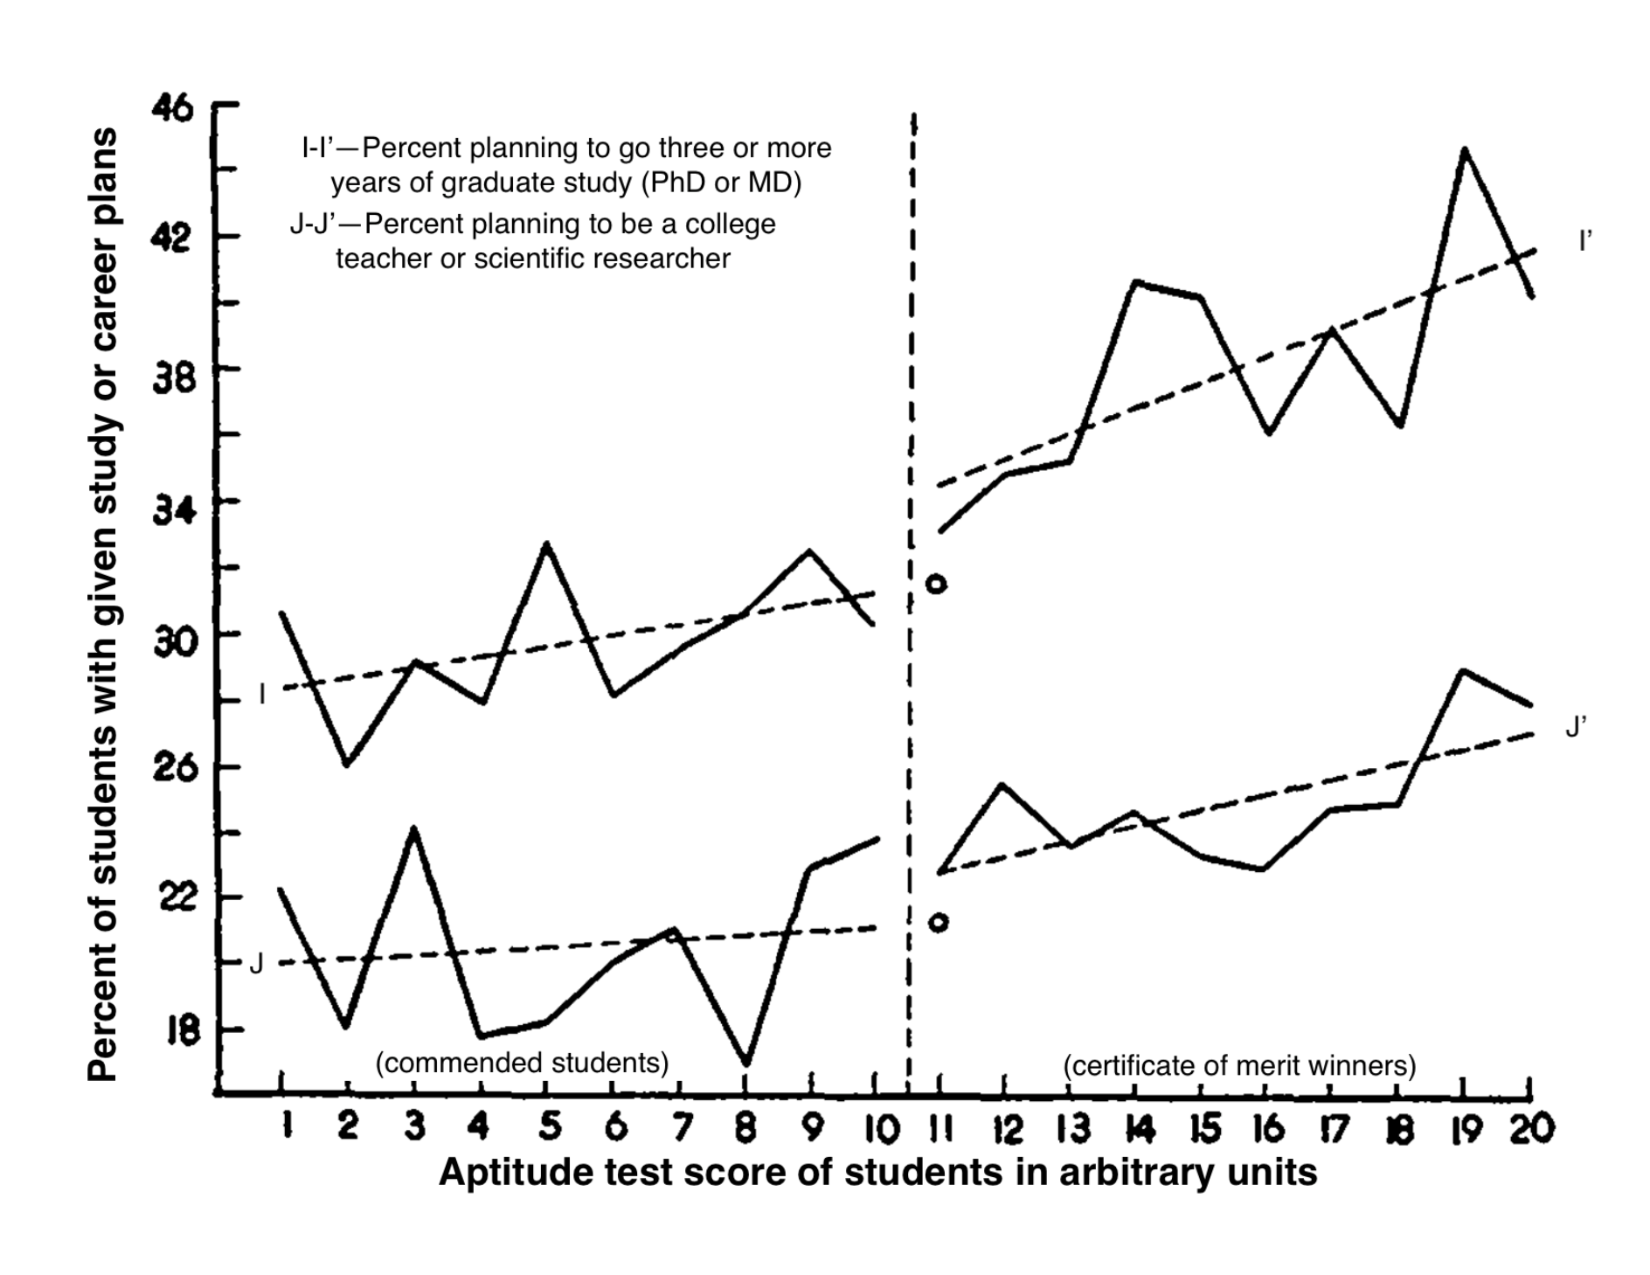
\includegraphics[width = \textwidth]{figures/rdd_graph_1960_modified.pdf}
\caption{A graph from \citet{thistlethwaite1960regression} with minor modifications of the unclear text in the original paper}\label{fig::thistlethwaite1960regression}
\end{figure}

 


\begin{example}
\citet{bor2014regression}  used regression discontinuity to study the effect of when to start HIV patients with antiretroviral on their mortality, where the treatment is determined by whether the patients' CD4 counts were below  200 cells/$\mu$L (note that CD4 cells are white blood cells that fight infection.)
\end{example}




\begin{example}
\citet{carpenter2009effect} studied the effect of alcohol consumption on mortality, which leverages the minimum legal drinking age as a discontinuity for alcohol consumption.  They derived mortality data from the National Center for Health Statistics,  including the decedent's date of birth and date of death. They computed the age profile of deaths per 100,000 person-years with outcomes measured by the following nine variables:
\begin{tabular}{cc}
\hline 
\texttt{all} & all deaths, the sum of  \texttt{internal} and \texttt{external}\\
\texttt{internal} & deaths due to internal causes\\
\texttt{external} & deaths due to external causes, the sum of the rest\\
\texttt{homicide} & homicides \\
\texttt{suicide} & suicides\\
\texttt{mva} & motor vehicle accidents\\
\texttt{alcohol} & deaths with a mention of alcohol\\
\texttt{drugs} & deaths with a mention of drug use\\
\texttt{externalother} & deaths due to other external causes\\
\hline 
\end{tabular}


Figure \ref{fig::mlda-9outcomes} plots the number of deaths per 100,000 person-years for nine measures based on the data used by \citet{angrist2014mastering}. From the jumps at age 21, it seems obvious that there is an increase in mortality at age 21, primarily due to motor vehicle accidents. I leave the formal analysis as Problem \ref{hw::MLDA}. 
\end{example}
 

\begin{figure}
\centering
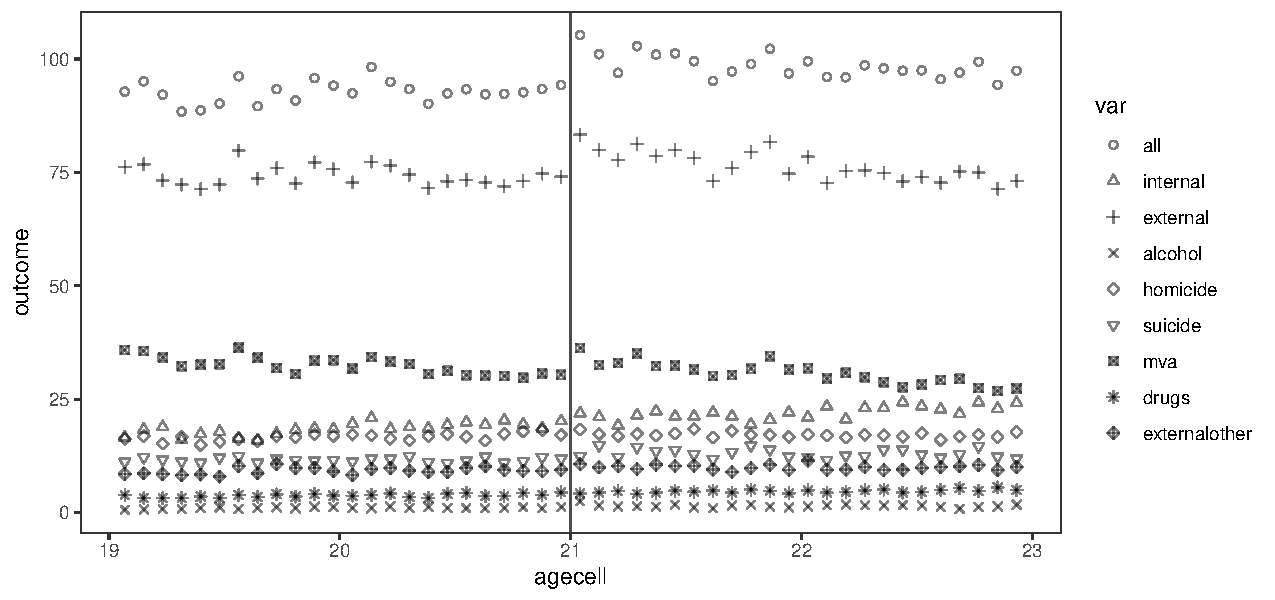
\includegraphics[width = \textwidth]{figures/mlda_9outcomes.pdf}
\caption{Minimum legal drinking age example from  \citet{carpenter2009effect}}\label{fig::mlda-9outcomes}
\end{figure}


 

 



\subsection{A mathematical formulation of regression discontinuity}


The technical term for the variable $X$ that determines the treatment is the {\it running variable}. 
Intuitively, regression discontinuity can identify a {\it local average causal effect} at the cutoff point $x_0$: 
$$
\tau(x_0) = E\{ Y(1) - Y(0)  \mid X=x_0 \}. 
$$
In particular, for the potential outcome under treatment, we have
\begin{eqnarray}
E\{ Y(1) \mid X=x_0 \} &=& \lim_{\varepsilon \rightarrow 0+ } E\{ Y(1) \mid X=x_0+\varepsilon \} \label{eq::srd-continuity} \\
&=& \lim_{\varepsilon \rightarrow 0+} E\{ Y(1) \mid Z=1, X=x_0+\varepsilon \}  \label{eq::srd-z} \\
&=&  \lim_{\varepsilon \rightarrow 0+} E( Y \mid Z=1, X=x_0+\varepsilon ),
\end{eqnarray} 
where \eqref{eq::srd-continuity} holds if $ E\{ Y(1) \mid X=x\}$ is continuous from the right at $x_0$ and \eqref{eq::srd-z} follows by the definition of $Z$. Similarly, for the potential outcome under control, we have
$$
E\{ Y(0) \mid X=x_0 \} =  \lim_{\varepsilon \rightarrow 0+} E( Y \mid Z=0, X=x_0-\varepsilon )
$$
if $ E\{ Y(0) \mid X=x\}$ is continuous from the left at $x_0$. 
So the local average causal effect at $x_0$ can be identified by the difference of the two limits. I summarize the key identification result below.


\begin{theorem}
\label{thm::identification-rdd}
Assume that the treatment is determined by  $Z = I(X \geq x_0)$
where $x_0$ is a predetermined threshold. 
Assume that $ E\{ Y(1) \mid X=x\}$ is continuous from the right at $x_0$ and $ E\{ Y(0) \mid X=x\}$ is continuous from the left at $x_0$. Then the local average treatment effect at $X=x_0$ is identified by
$$
\tau(x_0) = \lim_{\varepsilon \rightarrow 0+} E( Y \mid Z=1, X=x_0+\varepsilon ) - \lim_{\varepsilon \rightarrow 0+} E( Y \mid Z=0, X=x_0-\varepsilon ).
$$
\end{theorem}

Since the right-hand side of the above equation only involves observables, the parameter $\tau(x_0)$ is nonparametrically identified. However, the form of the identification formula is totally different from what we derived before. In particular, the identification formula involves limits of two conditional expectation functions. 



\subsection{Regressions near the boundary}\label{sec::rdd-numerical}

If we are lucky,  graphical diagnostics sometimes can clearly show the causal effect at the cutoff point. However, many outcomes are noisy so graphical diagnostics are not enough in finite samples. Figure \ref{fig::4examples-rdd} shows two simulated examples with obvious jumps at the cutoff point and two examples without obvious jumps, although the underlying data-generating processes all have discontinuities. 

\begin{figure}
\centering
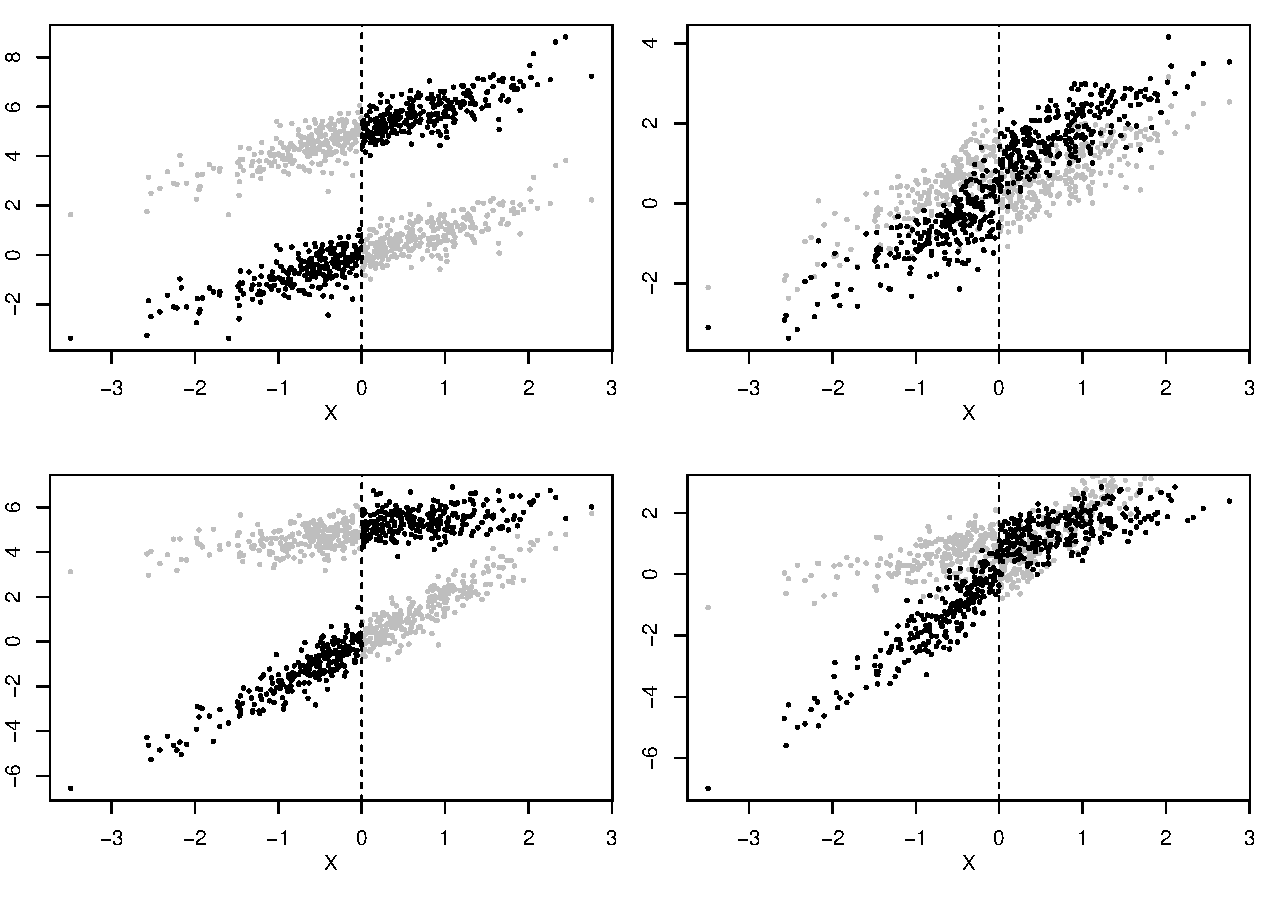
\includegraphics[width = \textwidth]{figures/rdd_graph.pdf}
\caption{Examples of regression discontinuity. The black points are the observed outcomes whereas the grey points are the unobserved counterfactual outcomes. 
In the first column, the data-generating processes result in visible jumps at the cutoff points; in the second column, the jumps are not so visible. In the first row, the data generating processes have constant $\tau(x)$; in the second row, $\tau(x)$ varies with $x$.  
}\label{fig::4examples-rdd}
\end{figure}



Assume that $E( Y \mid Z=1, X=x ) = \gamma_1 + \beta_1 x$ and $E( Y \mid Z=0, X=x ) = \gamma_0 + \beta_0 x $ are linear in $x$. We can run OLS based on the treated and control data to obtain the fitted lines $\hat\gamma_1 + \hat\beta_1 x$ and $\hat\gamma_0 + \hat\beta_0 x$, respectively. We can then estimate the average causal effect at the point $X = x_0$ as
$$
\hat\tau(x_0) = (\hat\gamma_1 -\hat\gamma_0 ) + (\hat\beta_1 -\hat\beta_0) x_0 .
$$
Numerically, $\hat\tau(x_0) $ is identical to the coefficient of $Z_i$ in the OLS
\begin{eqnarray}
Y_i \sim \{ 1, Z_i, X_i - x_0, Z_i (X_i - x_0)  \} , \label{eq::ols-rdd-1}
\end{eqnarray}
and it is also identical to the coefficient of $Z_i$ in the OLS
\begin{eqnarray}
Y_i \sim \{ 1, Z_i,  R_i, L_i \},\label{eq::ols-rdd-2}
\end{eqnarray}
where 
$$
R_i = \max(X_i - x_0, 0) ,\qquad L_i= \min (X_i - x_0, 0)
$$ 
indicate the right and left parts of  $X_i - x_0$, respectively. I leave the algebraic details to Problem \ref{hw::rdd-ols-fits}.


However, this approach may be sensitive to the violation of the linear model assumption. Theory suggests running regression using only the local observations near the cutoff point\footnote{This is called {\it local linear regression} in nonparametric statistics, which belongs to a broader class of {\it local polynomial regression} \citep{fan2018local}. }. However, the rules for choosing the ``local points'' are quite involved. Fortunately, the \ri{rdrobust} function in the \ri{rdrobust} package in \ri{R} implements various choices of  ``local points.'' Since choosing the ``local points'' is the key to regression discontinuity, it seems more sensible to report estimates and confidence intervals based on various choices of the ``local points.'' This can be viewed as a sensitivity analysis for regression discontinuity. 


\subsection{An example}
\label{section::lee-RDD-example}

\citet{lee2008randomized} gave a famous example of using regression discontinuity to study the incumbency advantage in the U.S. House. 
He wrote that ``incumbents are, by definition, those politicians who were successful in the previous election. If what makes them successful is somewhat persistent over time, they should be expected to be somewhat more successful when running for re-election.'' Therefore, this is a fundamentally challenging causal inference problem. The regression discontinuity is a clever study design to study this problem. 



The running variable is the lagged vote in the previous election centered at $0$, and the outcome is the vote in the current election, with units being the congressional districts. The treatment is the binary indicator for being the current incumbent party in a district, determined by the lagged vote. The following \ri{R} code generates  Figure \ref{fig::lee2008} that shows the raw data. 

\begin{lstlisting}
house = read.csv("house.csv")[, -1]
plot(y ~ x, data = house, pch = 19, cex = 0.1)
abline(v = 0, col = "grey")
\end{lstlisting}

\begin{figure}
\centering
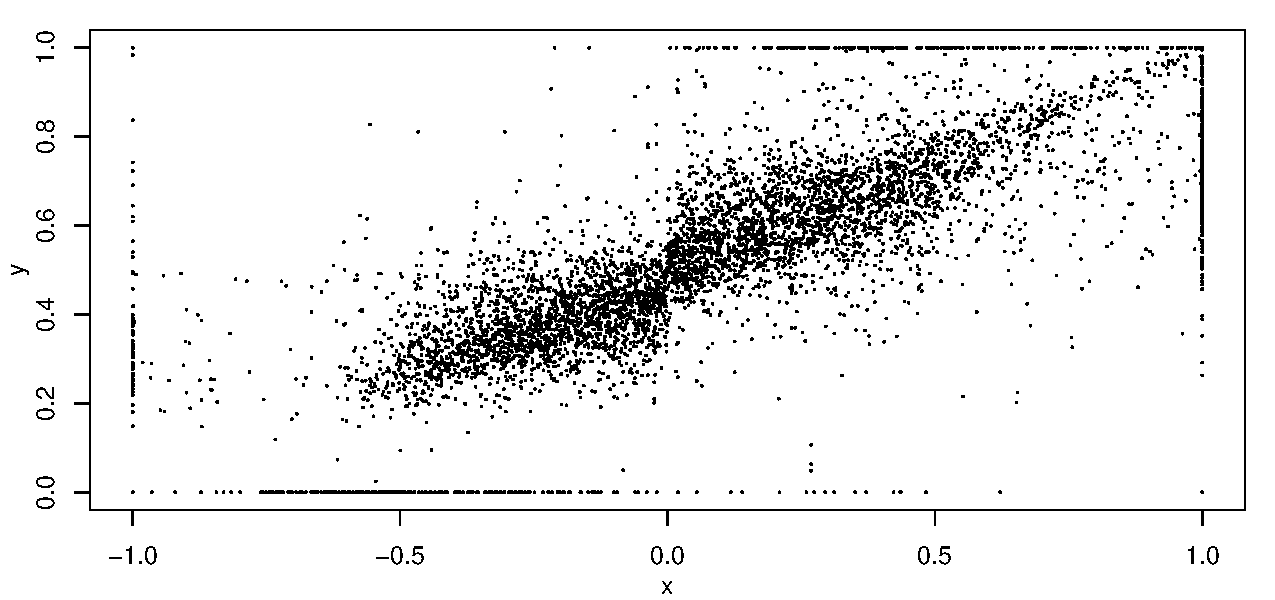
\includegraphics[width = \textwidth]{figures/lee2008rdd.pdf}
\caption{Raw data of \citet{lee2008randomized} }\label{fig::lee2008}
\end{figure}

 
The \ri{rdrobust} function gives three sets of the point estimate and confidence intervals. They all suggest a positive incumbency advantage. 

\begin{lstlisting}
> library(rdrobust)
> RDDest = rdrobust(house$y, house$x)
Warning message:
In rdrobust(house$y, house$x) :
  Mass points detected in the running variable.
> cbind(RDDest$coef, RDDest$ci)
                    Coeff   CI Lower   CI Upper
Conventional   0.06372533 0.04224798 0.08520269
Bias-Corrected 0.05937028 0.03789292 0.08084763
Robust         0.05937028 0.03481238 0.08392818
\end{lstlisting}
 
 
 
We can also obtain the point estimates and the confidence intervals based on OLS with different choices of the local points defined by $|X| < h$ based on the following \ri{R} code.
\begin{lstlisting}
house$z = (house$x >= 0)
hh = seq(0.05, 1, 0.01)
local.lm = sapply(hh, function(h){
  Greg = lm(y ~ z + x + z*x, data = house,
            subset = (abs(x)<=h))
  cbind(coef(Greg)[2], confint(Greg, 'zTRUE'))
})
plot(local.lm[1, ] ~ hh, type = "p",
     pch = 19, cex = 0.3,
     ylim = range(local.lm),
     xlab = "h",
     ylab = "point and interval estimates",
     main = "subset linear regression: |X|<h")
lines(local.lm[2, ] ~ hh, type = "p",
      pch = 19, cex = 0.1) 
lines(local.lm[3, ] ~ hh, type = "p",
      pch = 19, cex = 0.1)
\end{lstlisting}
Figure \ref{fig::rdd-lee} shows the point estimates and the confidence intervals as a function of $h$. While the point estimates and the confidence intervals are sensitive to the choice of $h$, the qualitative result remains the same as above. 
 
\begin{figure}[h]
\centering
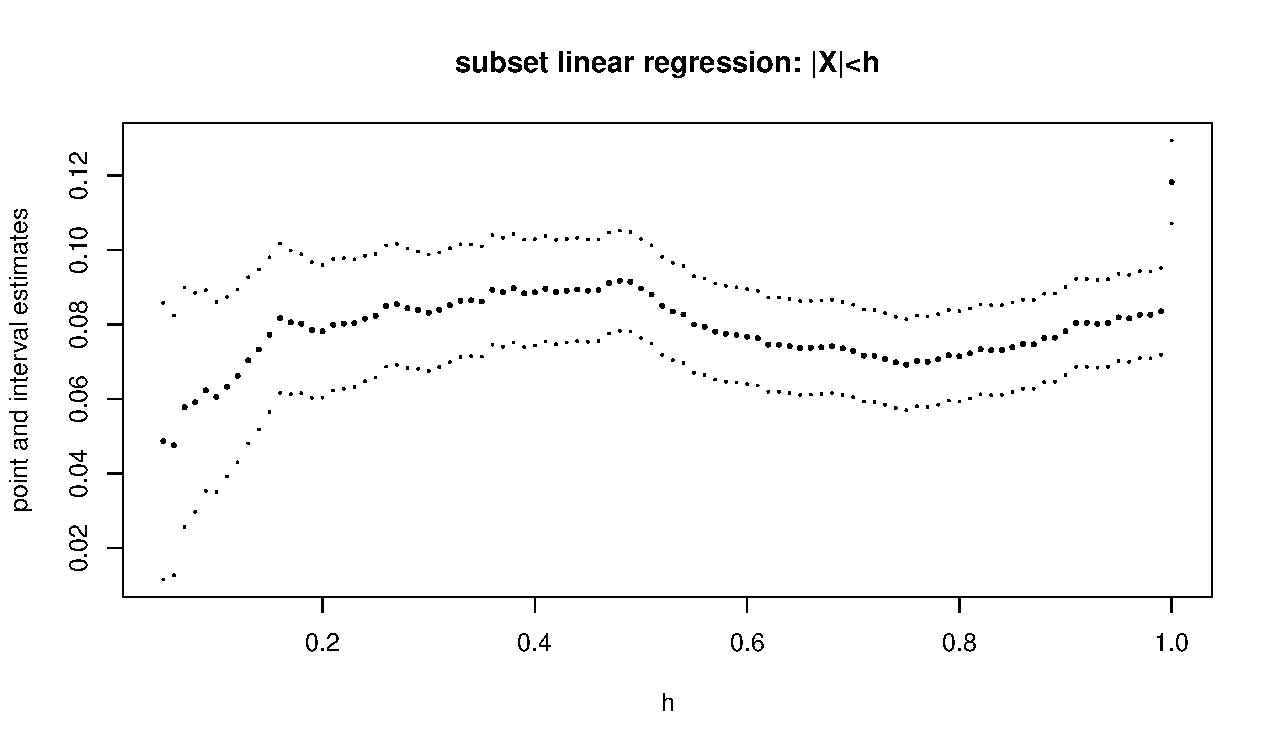
\includegraphics[width = \textwidth]{figures/rdd_lee.pdf}
\caption{Estimates and confidence intervals based on local linear regressions}\label{fig::rdd-lee}
\end{figure} 
 
 
 
\subsection{Problems of regression discontinuity}\label{sec::problems-RD}


What can go wrong with the regression discontinuity analysis? The technical challenge is to specify the neighborhood near the cutoff point. We have discussed this issue above.

In addition, Theorem \ref{thm::identification-rdd} holds under a continuity condition. It may be violated in practice. For instance, if the mortality rate jumps at the age of 21, then we may not be able to attribute the jumps in Figure \ref{fig::mlda-9outcomes} to the change in drinking behavior due to the legal drinking age. However, it is hard to check the violation of the continuity condition empirically.
 
 
\citet{mccrary2008manipulation} proposed an indirect test for the validity of the regression discontinuity. He suggested checking the density of the running variable at the cutoff point. The discontinuity in the density of the running variable at the cutoff point may suggest that some units were able to manipulate their treatment status perfectly. The \ri{DCdensity} function in the \ri{R} package \ri{rdd} implements this test. I omit the details. 


 
 
\section{Homework Problems}

 

\paragraph{A theorem for the role of outcome modeling in the presence of limited overlap}\label{hw::outcome-modeling-overlap}

This problem extends the discussion in Section \ref{sec::outcome-modeling-overlap}. I state a formal theorem below.

\begin{theorem}
\label{thm::outcome-overlap}
Assume 
$$
Z\ind Y(z) \mid X, \quad (z=0,1)
$$
and
$$
E\{  Y(z) \mid X \} = f_z( r(X)   ),\quad (z=0,1)
$$
for some function $r(X)$. 
The average causal effect $\tau = E\{ Y(1) - Y(0)  \}$ can be identified by
$$
\tau =E\{   E(Y\mid Z=1, r(X)) - E(Y\mid Z=0, r(X)) \} 
$$
or
$$
\tau = E\left\{   \frac{ZY}{  e(r(X)) }  \right\}  - E\left\{   \frac{(1-Z)Y}{ 1 -  e(r(X)) }  \right\}
$$
where $e(r(X)) = \pr\{ Z=1\mid r(X) \}$. 
\end{theorem}

Prove Theorem \ref{thm::outcome-overlap}.

Remark: When $r(X) = X$, Theorem \ref{thm::outcome-overlap} reduces to the standard IPW formula for the average causal effect. When $r(X)$ has a lower dimension than $X$, Theorem \ref{thm::outcome-overlap} has broader applicability if the overlap condition on $e(X)$ fails whereas the overlap condition on $e(r(X)) $ may still hold. 




 \paragraph{Linear potential outcome models}\label{hw::rdd-ols-fits}
 
 
 This problem gives more details for the numerical equivalence in Section \ref{sec::rdd-numerical}. 
 
 Show that $\hat\tau(x_0) $ equals the coefficients of $Z_i$ in OLS fits \eqref{eq::ols-rdd-1} and \eqref{eq::ols-rdd-1}. 
 
% Assume that 
% $$
% Y_i(1) = \gamma_1 + \beta_1 X_i + \varepsilon_i(1),\quad
%  Y_i(0) = \gamma_0 + \beta_0 X_i + \varepsilon_i(0)
% $$
%with $ E\{\varepsilon_i(1) \mid X_i \} =  E\{\varepsilon_i(0) \mid X_i \} = 0$. First, express 
%$$
%\tau(x_0) = E\{ Y_i(1) - Y_i(0)\mid X_i = x_0 \} 
%$$ 
%in terms of the parameters in the above model, and then show that $\tau(x_0)$ can be unbiased estimated by the coefficient of $Z_i$ in the OLS fits of \eqref{eq::ols-rdd-1} or \eqref{eq::ols-rdd-2}.  


Remark: It is helpful to start with the figures of $Z_i(X_i - x_0)$, $L_i$, and $R_i$ with $X_i$ on the x-axis. The conclusion holds by a reparametrization of the OLS regressions. 



\paragraph{Simulation for regression discontinuity}

In Figure \ref{fig::4examples-rdd}, the potential outcomes are simulated from linear models. Change them to nonlinear models, and compare different point estimators and confidence intervals, including the biases and variances of the point estimators, and the coverage properties of confidence intervals. 



\paragraph{Re-analysis of the data on the minimum legal drinking age}\label{hw::MLDA}


Figure \ref{fig::mlda-9outcomes} shows the jumps at the cutoff point. 
Analyze the data \ri{mlda.csv} of \citet{carpenter2009effect}.

\paragraph{Re-analysis of \citet{lee2008randomized}'s data}\label{hw::lee2008-robust}

Figure \ref{fig::rdd-lee} plots the confidence intervals based on the standard errors assuming homoskedasticity. Generate a figure with confidence intervals based on the EHW standard errors in OLS. 




\paragraph{Recommended reading}

\citet{d2017overlap} discussed the implications of overlap with high dimensional covariates. 

\citet{thistlethwaite1960regression}'s original paper on regression discontinuity was re-printed as \citet{thistlewaiteregression2016obs} with many insightful comments.  Coincidentally, \citet{thistlethwaite1960regression} and \citet{Rubin:1974} were both published in the {\it Journal of Educational Psychology}.
